%%=============================================================================
%% Methodologie
%%=============================================================================
\chapter{Methodologie}
\label{ch:methodologie}

%% TODO: Hoe ben je te werk gegaan? Verdeel je onderzoek in grote fasen, en
%% licht in elke fase toe welke stappen je gevolgd hebt. Verantwoord waarom je
%% op deze manier te werk gegaan bent. Je moet kunnen aantonen dat je de best
%% mogelijke manier toegepast hebt om een antwoord te vinden op de
%% onderzoeksvraag.

Nu de vereisten van Kayzr gekend zijn, kan het ontwerpen van de middleware toepassing van start gaan. Hiervoor zal er een bepaalde werkwijze worden gehanteerd, waarover zo dadelijk meer uitleg wordt gegeven. Tijdens het ontwerpen van de middleware zal echter niet enkel met Kayzr's requirements rekening gehouden worden. Het is de bedoeling dat dit geen hardcoded stuk software in Kayzr's backend wordt, maar een abstracte, universele middleware dat gedownload en geïnstalleerd kan worden via Node.js package manager.  

\section{Werkwijze}
\label{sec:werkwijze}

Men is als volgt te werk gegaan: eerst werd een middleware ontwikkeld dat op een mooie manier elke request kon loggen in de console. Erna werd een server aangemaakt op één van de servers van Kayzr, en werd daar Grafana en InfluxDB op geïnstalleerd. Tenslotte werd de middleware geabstraheerd, waarna er getracht werd om connectie te maken met de databank en telkens na een bepaald interval, data naar InfluxDB weg te schrijven. Wanneer de data van de middleware tenslotte Grafana bereikte, werd de middleware geïnstalleerd op Kayzr's backend. Op het einde werden er dan grafieken aangemaakt in Grafana die de requirements van Kayzr zouden volbrengen. 

\subsection{Multilogger}
\label{sec:multilogger}

De te ontwikkelen middleware werd omgedoopt tot Multilogger (en later officieel express-influx-multilogger). Als eerste werd een basis express applicatie aangemaakt, waarin de eerste stapjes middleware software werden geschreven. Als eerste werd er geprobeerd om per keer dat een API call werd gemaakt, de methode van deze call naar de console te loggen.

In app.js
\begin{lstlisting}[language=JavaScript, breaklines=true, numbers=left, frame=single, caption={app.js eerste stap},label=code:appjsFirst]
var app = express();

app.use(bodyParser.json());
app.use(bodyParser.urlencoded({ extended: true }));
app.use(express.static(path.join(__dirname, 'public')));

app.use(multilogger.multilog); // Custom middleware

app.use('/', indexRouter);

app.listen(3000);
\end{lstlisting}

In multilogger.js
\begin{lstlisting}[language=JavaScript, breaklines=true, numbers=left, frame=single, caption={multilogger.js eerste stap},label=code:multilogFirst]
const multilogger = {
	multilog: (req, res, next) => {
	console.log('\n=====- Multilogger v0.1 -=====');
	console.log('--- Basic ---\n');
	
	res.on('finish', () => {
		console.info(`${req.method} --- ${res.statusCode} ---  ${res.statusMessage}  at ${new Date().toLocaleString()}`);
		console.info(`Response-time: ${res.getHeader('X-Response-Time')}`);
		console.info(`URL: ${req.hostname} --- ${req.url}`);
		console.info(`Client: ${req.ip} --- ${req.header('User-Agent')}`);
	});
	

	next();
	},
};

module.exports = multilogger; 
\end{lstlisting}

Dit werd uiteindelijk meer uitgebreid, zodat er een mooi breed overzicht naar de console werd gelogd. Natuurlijk wensen niet alle ontwikkelaars dat er per API all naar de console zou worden gelogd met zeer veel overbodige informatie, aangezien dit kan oplopen van (uiteraard afhankelijk van de software) honderden tot duizenden calls per enkele seconden. Daarom werd er een parameter toegevoegd om deze functionaliteit uit te schakelen, met in het achterhoofd dat de middleware niet enkel zou dienen voor een mooi console-overzicht te geven. Dit was een nice-to-have-functionaliteit voor Kayzr, maar was wel een noodzakelijke eerste stap om op verder te bouwen. Ook werd er een aangepaste \textit{error handler} (stuk code dat fouten afhandelt die zich voortdoen tijdens een API call) geschreven, waardoor ook foutberichten konden gelogd worden.

\begin{lstlisting}[language=JavaScript, breaklines=true, numbers=left, frame=single, caption={Parameters toegevoegd},label=code:multilogparams]
app.use(multilogger.log({ development: false, extended: false }));
\end{lstlisting}

\begin{lstlisting}[language=JavaScript, breaklines=true, numbers=left, frame=single, caption={MultiError.js, de custom error handler},label=code:multiError]
const throwMultilogError = () => {
	return (err, req, res, next) => {
		if (!err) {
			return next();
		}
		res.locals.multiError = {
			errorMessage: err.message,
			errorStack: err.stack
		};
		next();
	};
};

module.exports = throwMultilogError;
\end{lstlisting}

\subsection{Grafana en InfluxDB}
\label{sec:grafanaAndInflux}

Vervolgens moest er een systeem gekozen worden om verzamelde data op te slaan en weer te geven. Dit kan natuurlijk gerealiseerd worden met verschillende databanken en frontend frameworks. Origineel werd er geopteerd om gebruik te maken van MySQL samen met een React.js applicatie om de data te visualiseren, maar na verder onderzoek bleek dat hier reeds handigere software voor bestaat, namelijk InfluxDB, en Grafana, dixit \textcite{Hill2015}. InfluxDB is een snelle, open source time series database, gemaakt om op een snelle manier data zoals metrieken en events op te slaan, gebonden doorheen een tijdsperiode. Grafana daarentegen, is een open platform om time series data om te zetten in prachtige grafieken. Het spreekt dan ook voor zich dat deze twee hand in hand gaan.

Er werd een server van Kayzr toegewezen om dit te testen. Hiervoor werden via Docker twee containers aangemaakt (een soort van virtuele omgeving om deze software op te laten draaien), en werden tenslotte toegewezen aan InfluxDB en Grafana. Uiteindelijk werd de server opgestart, werd Grafana geïnstalleerd en geïnitialiseerd en werd de (lege) Influx-databank gekoppeld. 

\subsection{Wegschrijven en abstraheren}
\label{sec:abstraction}
Nu dat de databank was aangemaakt, werd het tijd om deze te koppelen aan de middleware. Gebaseerd op het voorgaande logsysteem, werd een object aangemaakt dat alle belangrijke info zou bevatten. 

\begin{lstlisting}[language=JavaScript, breaklines=true, numbers=left, frame=single, caption={Log object},label=code:multilogLogObject]
const object = {
	method: req.method,
	statusCode: res.statusCode,
	statusMessage: res.statusMessage,
	date: new Date().toUTCString(),
	responseTime: elapsedTimeInMs,
	contentType: req.header("Content-Type") || " ",
	hostname: req.hostname,
	url: req.url,
	path: res.statusCode !== 404 && req.route && req.route.path ? req.route.path : "No Path",
	body: req.method === "POST" ? realBody : " ",
	params: _.isEmpty(req.params) ? " " : JSON.stringify(req.params),
	query: _.isEmpty(req.query) ? " " : JSON.stringify(req.query),
	cookies: _.isEmpty(req.cookies) ? " " : JSON.stringify(req.cookies),
	auth: req.header("Authorization") || req.header("x-access-token") || " ",
	ip: req.connection.remoteAddress,
	location: location,
	clientInfo: req.header("User-Agent") || " ",
	memoryUsage: memoryUsage,
	cpuUsage: cpuUsage,
	errorMessage: res.locals.multiError || " "
};

\end{lstlisting}

Via een reeds bestaande npm package, namelijk \href{https://github.com/node-influx/node-influx}{\textit{node influx}}, werd dit snel opgelost. Er werd een schema ontwikkeld waaruit optimaal de data zou kunnen geformatteerd worden naar Grafana, en niet veel later vloeiden de eerste metrieken Grafana binnen. Tenslotte werd er een buffer geïmplementeerd, dat om een gegeven interval de opgeslagen data wegschrijft en zichzelf weer leegt voor het volgende interval. 

De volgende stap in het ontwikkelen van een middleware oplossing voor Kayzr, was het abstraheren van de code. Zo kan niet enkel Kayzr hiervan gebruik maken, maar echter iedereen met een Node.js en Express configuratie. Er kwamen wat moeilijkheden opduiken bij het loskoppelen van de code, maar uiteindelijk werd er een abstracte, logische en schaalbare middleware geschreven volgens de richtlijnen van npm. Via parameters kan een gebruiker de functionaliteiten van de middleware aanpassen, en er werd ook ruimte voorzien om later extra database management systemen toe te voegen. De middleware werd omgedoopt tot express-influx-multilogger, werd open source gemaakt en werd uiteindelijk op npm gepubliceerd. Als laatste werd deze gloednieuwe package dan binnengetrokken op de backend en frontend van Kayzr's webplatform. Zo geraakte influx op een snellere manier gevuld met relevante data zodat er begonnen kon worden met het ontwikkelen van de volgende stap. 

\subsection{Grafana's grafieken}
\label{sec:graphs}

Als allerlaatste, werd Grafana opgebouwd om mooie relevante grafieken weer te geven aan de eindgebruiker. De verzamelde data bleek niet altijd even relevant of goed genoeg te zijn om er een grafiek mee op te bouwen, dus was er regelmatig een noodzaak om weer naar de vorige stap terug te gaan en het schema van InfluxDB aan te herzien. Hierdoor kwamen ook nieuwe ideeën tot stand, zoals het toevoegen van een gebruiker zijn geolocatie en het monitoren van de snelheid van elk databank verzoek per API call. Op het moment van schrijven zijn er in Grafana 7 grafieken te bezichtigen.

\subsubsection{Basics}
\label{sec:basics}
Hier worden de basis headers van elke API call getoond. De data bestaat uit een timestamp, ip-adres, response time, host, statuscode, statusbericht, methode, url, pad, en body. 

\begin{figure}[h]
	\centering
	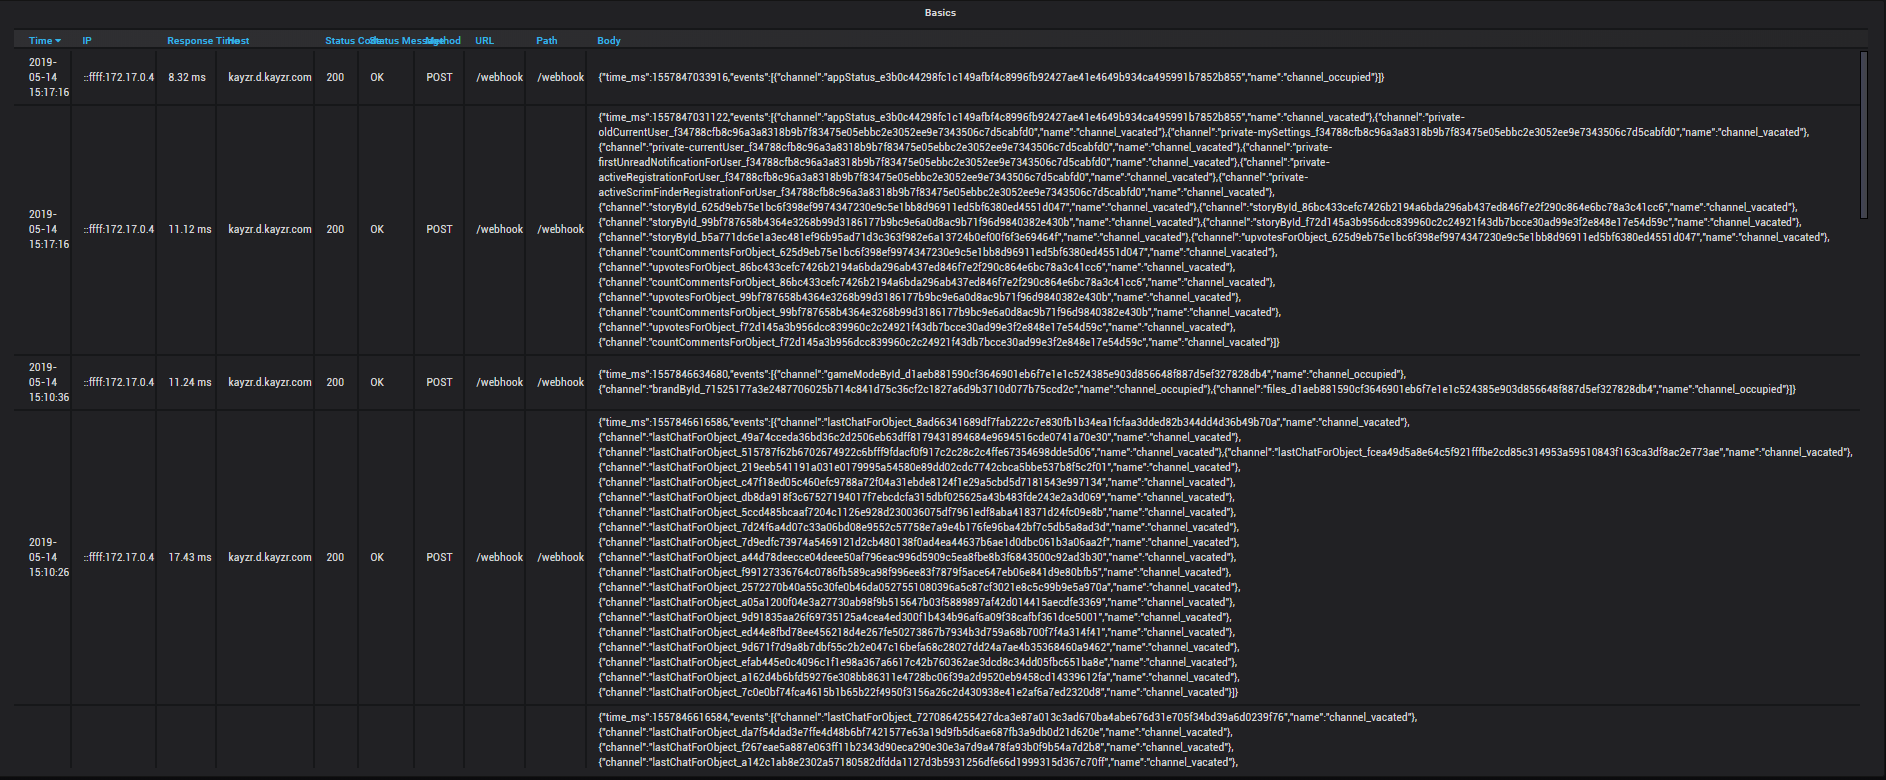
\includegraphics[width=\linewidth]{basics.png}
	\caption{Basics-paneel}
	\label{fig:basics}
\end{figure}

\subsubsection{Number of requests}
\label{sec:numberofrequests}
Het aantal verzoeken in een gegeven tijdsframe. Ook kunnen deze opgesplitst worden per statuscode, zodat men bijvoorbeeld kan observeren hoeveel API calls een fout gaven.

\begin{figure}[h]
	\centering
	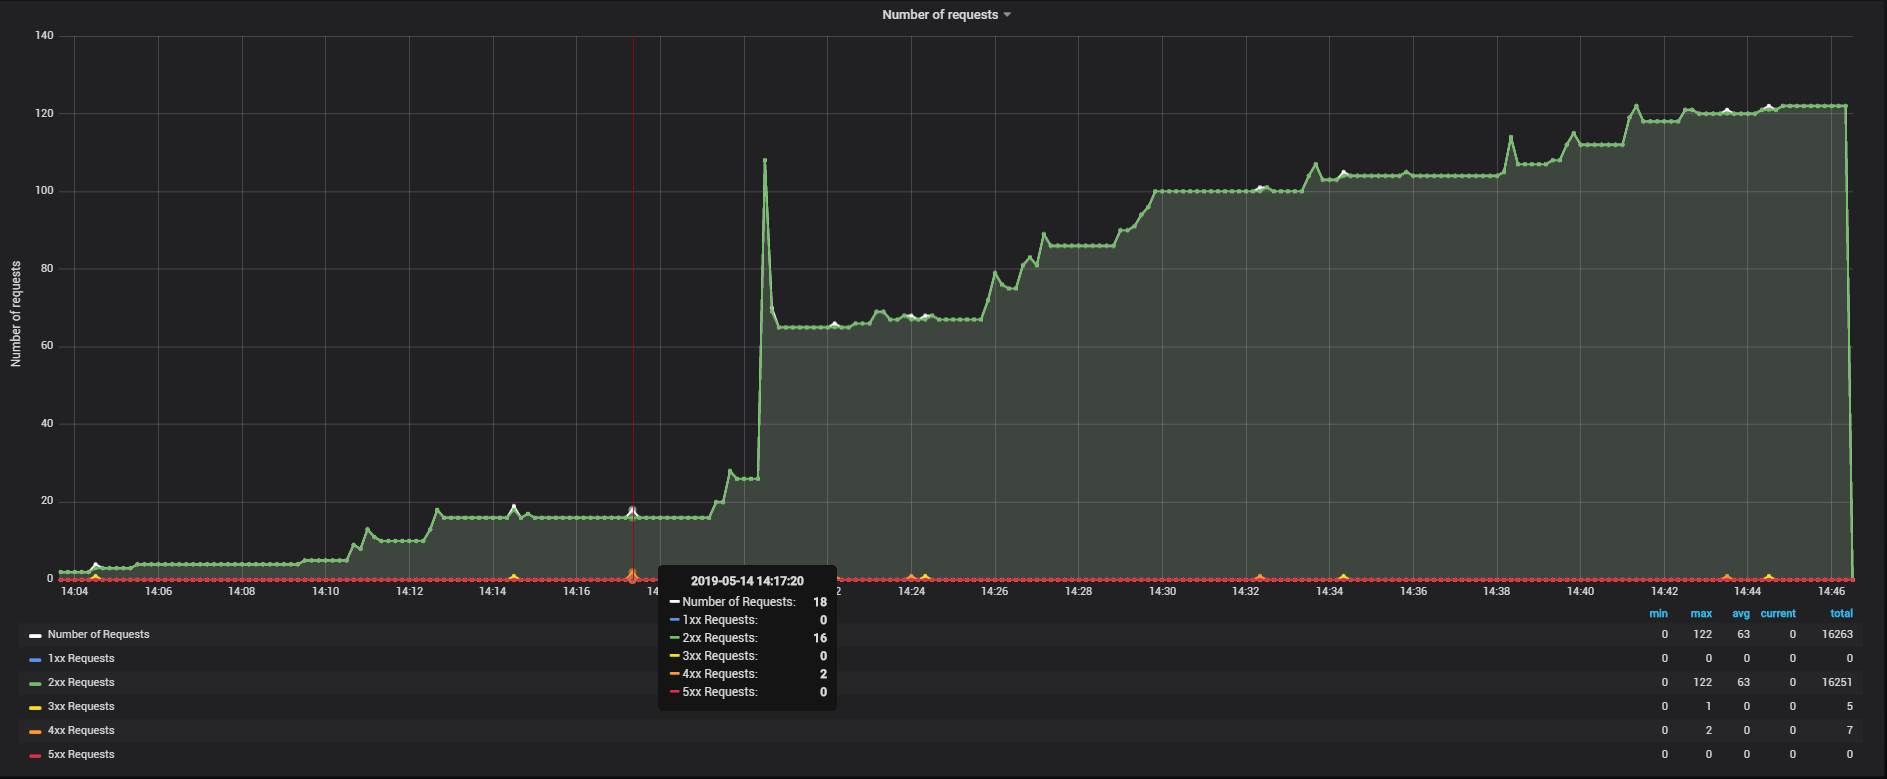
\includegraphics[width=\linewidth]{requests.png}
	\caption{Aantal requests-paneel (wit voor totaal, blauw voor requests dat starten met 1xx, groen voor 2xx, geel voor 3xx, oranje voor 4xx en rood voor 5xx.)}
	\label{fig:requests}
\end{figure}

\subsubsection{Errors}
\label{sec:errors}
Hier worden de foutmeldingen getoond, gegroepeerd per unieke foutmelding. Naast een timestamp, foutmelding en de error stack, worden ook de host, status, url en path weergeven. Aangezien Kayzr dit ook wou gebruiken voor debug-doeleinden, worden ook de body en authenticatietokens weergeven.

\begin{figure}[h]
	\centering
	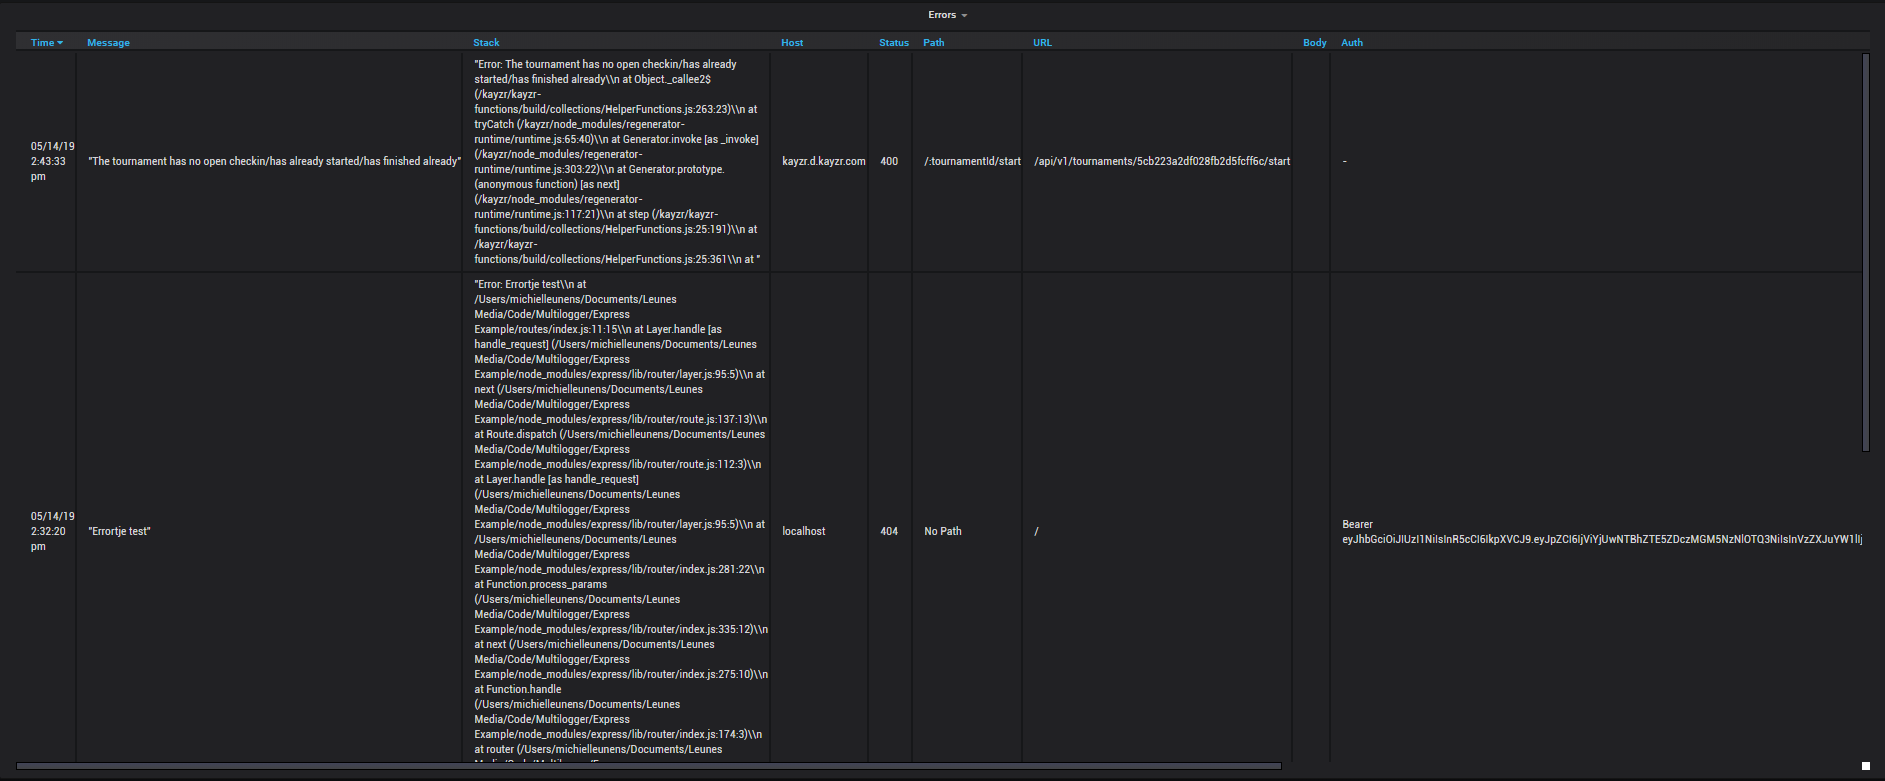
\includegraphics[width=\linewidth]{errors.png}
	\caption{Errors-paneel}
	\label{fig:errors}
\end{figure}

\subsubsection{Database timings}
\label{sec:dbtimings}
Hier wordt per API call de tijden gelogd van een bepaald verzoek naar de databank. Zo kan men per call zien hoeveel tijd het vraag om specifieke data op te halen.

%\begin{figure}[h]
%	\centering
%	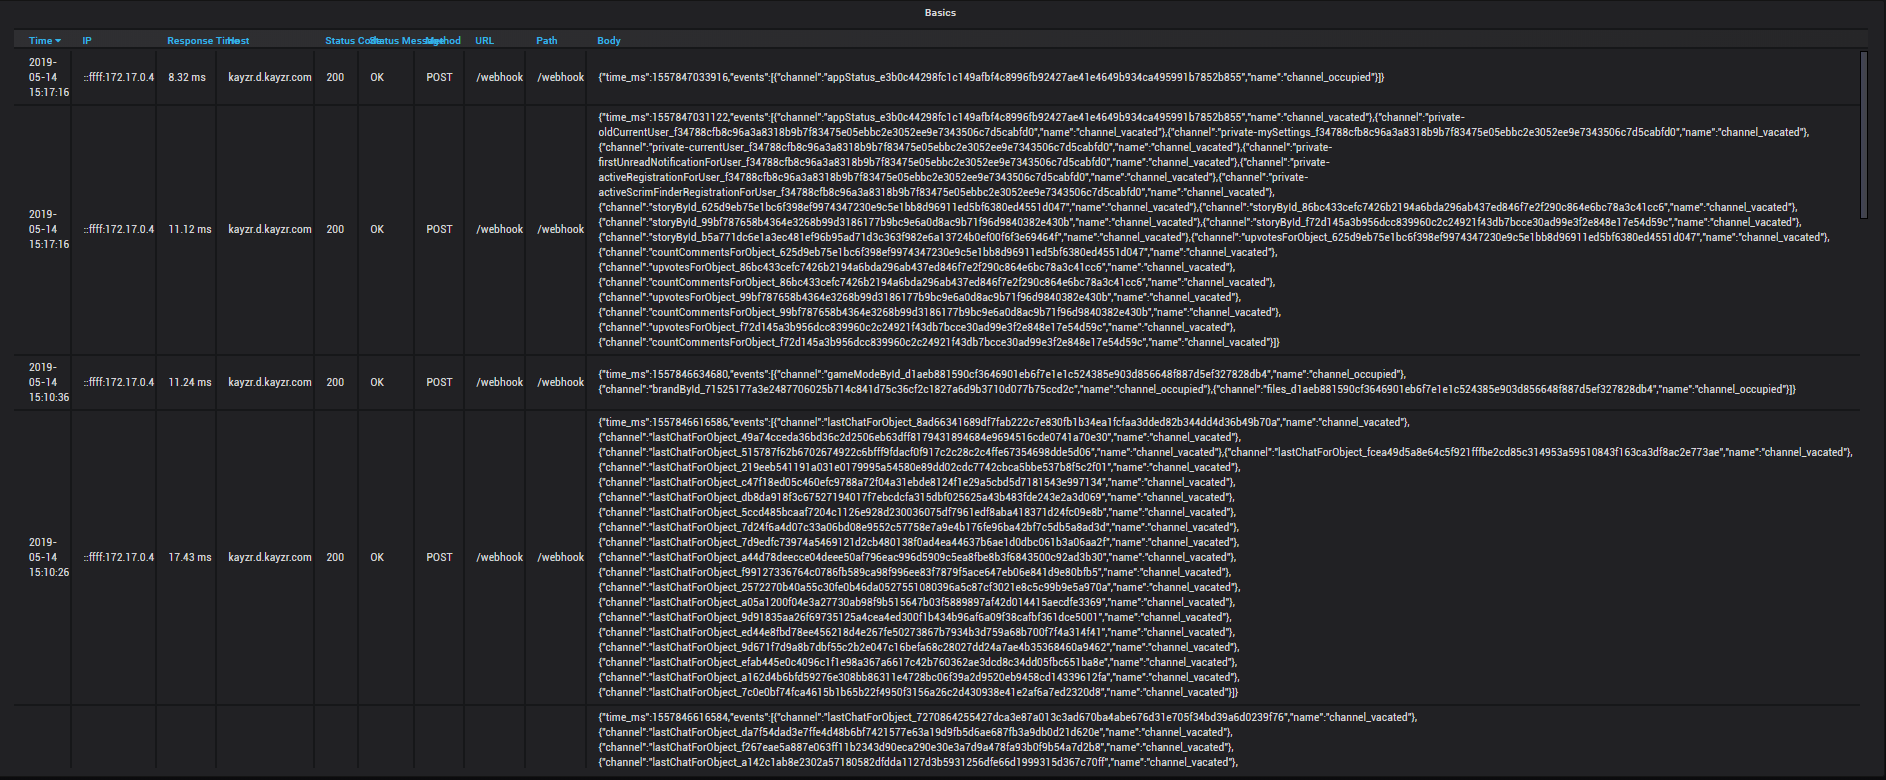
\includegraphics[width=\linewidth]{basics.png}
%	\caption{Basics-paneel}
%	\label{fig:basics}
%\end{figure}

\subsubsection{Users}
\label{sec:users}
Op een wereldkaart wordt het aantal gebruikers per land getoond. De geolocatie wordt afgeleid van het ip-adres van de gebruiker, en specifieke locaties worden dus niet opgevraagd.

\begin{figure}[h]
	\centering
	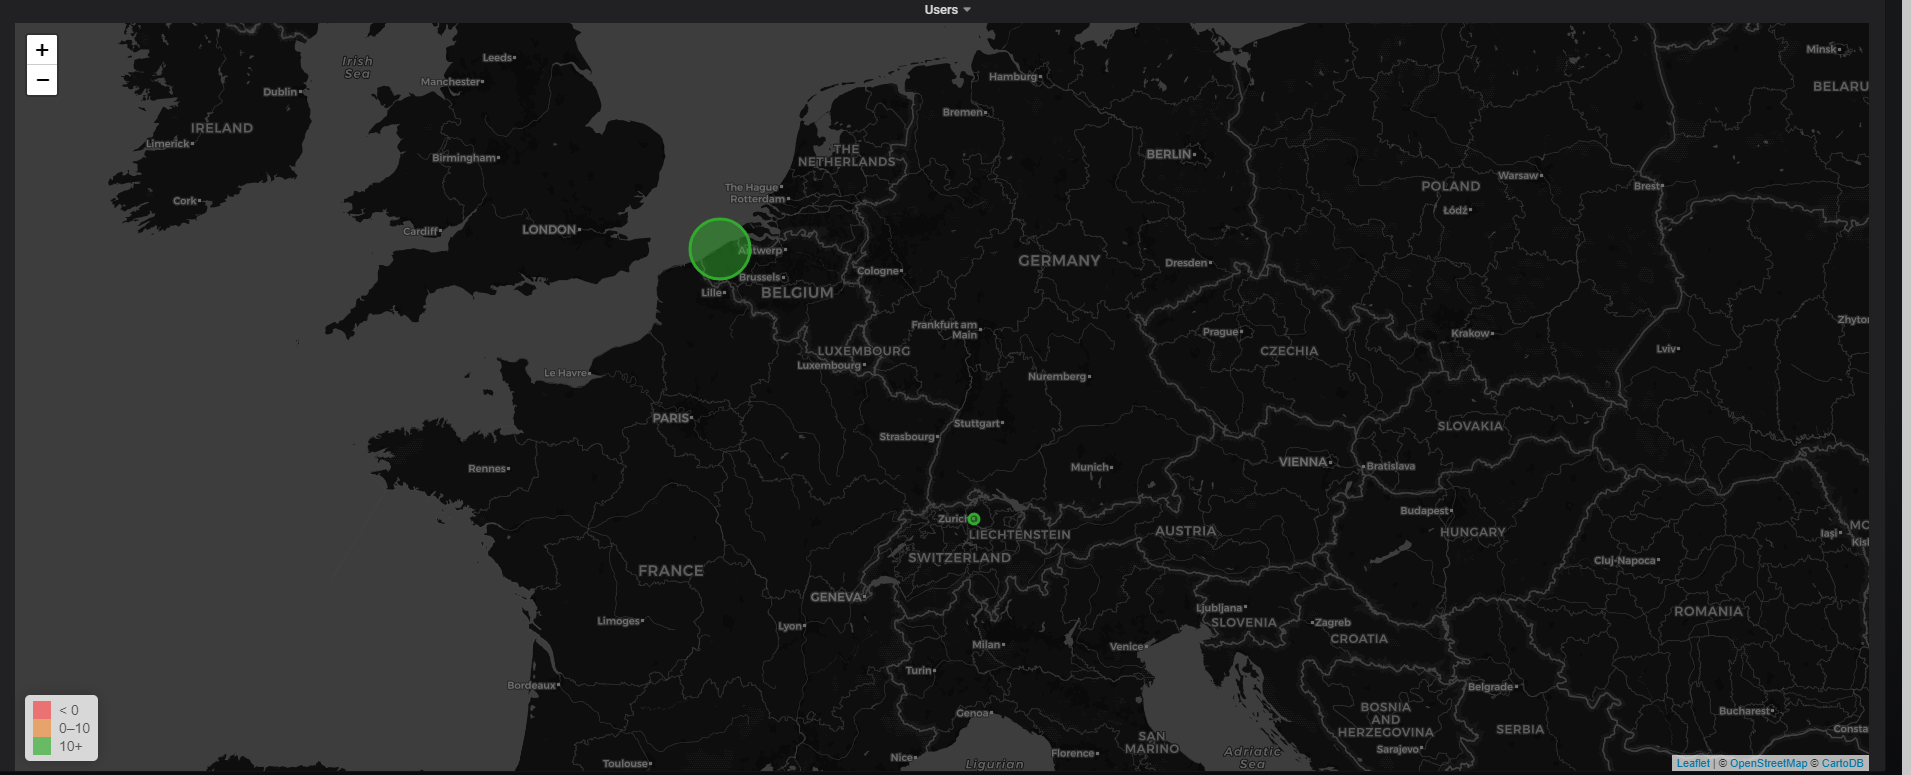
\includegraphics[width=\linewidth]{users.png}
	\caption{Users-paneel}
	\label{fig:users}
\end{figure}

\subsubsection{Memory Usage}
\label{sec:memory}
Het geheugenverbruik per gigabyte van de machine waarop de server draait.
\begin{figure}[h]
	\centering
	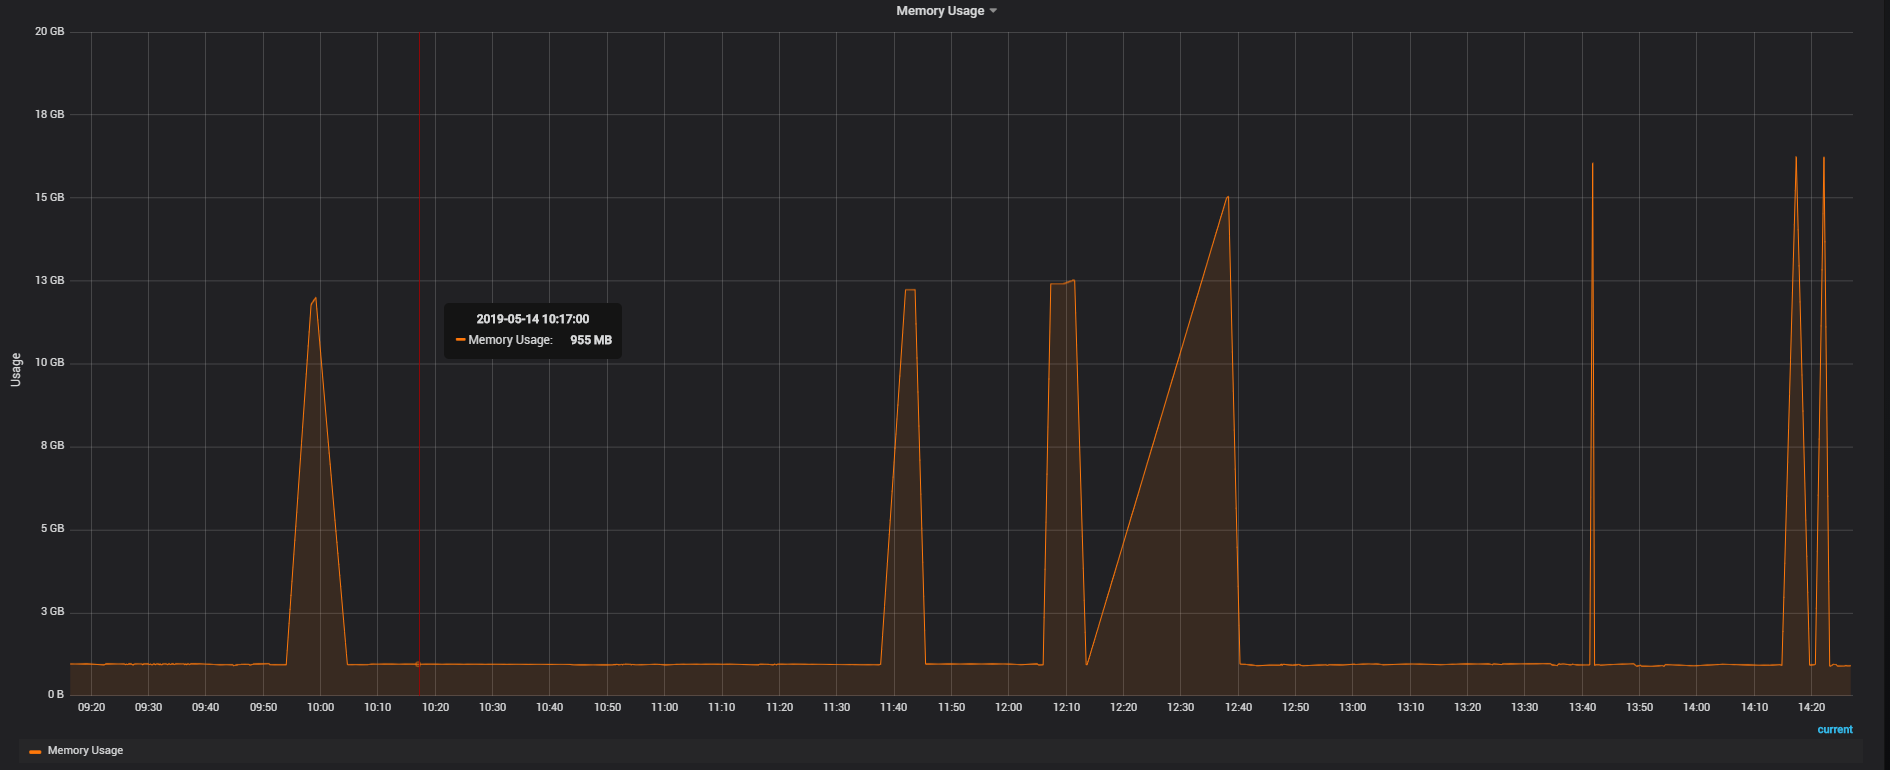
\includegraphics[width=\linewidth]{memory.png}
	\caption{Geheugenverbruik-paneel}
	\label{fig:mem}
\end{figure}

\subsubsection{CPU Usage}
\label{sec:cpu}
Het processorverbruik in percentages van de machine waarop de server draait.

\begin{figure}[h]
	\centering
	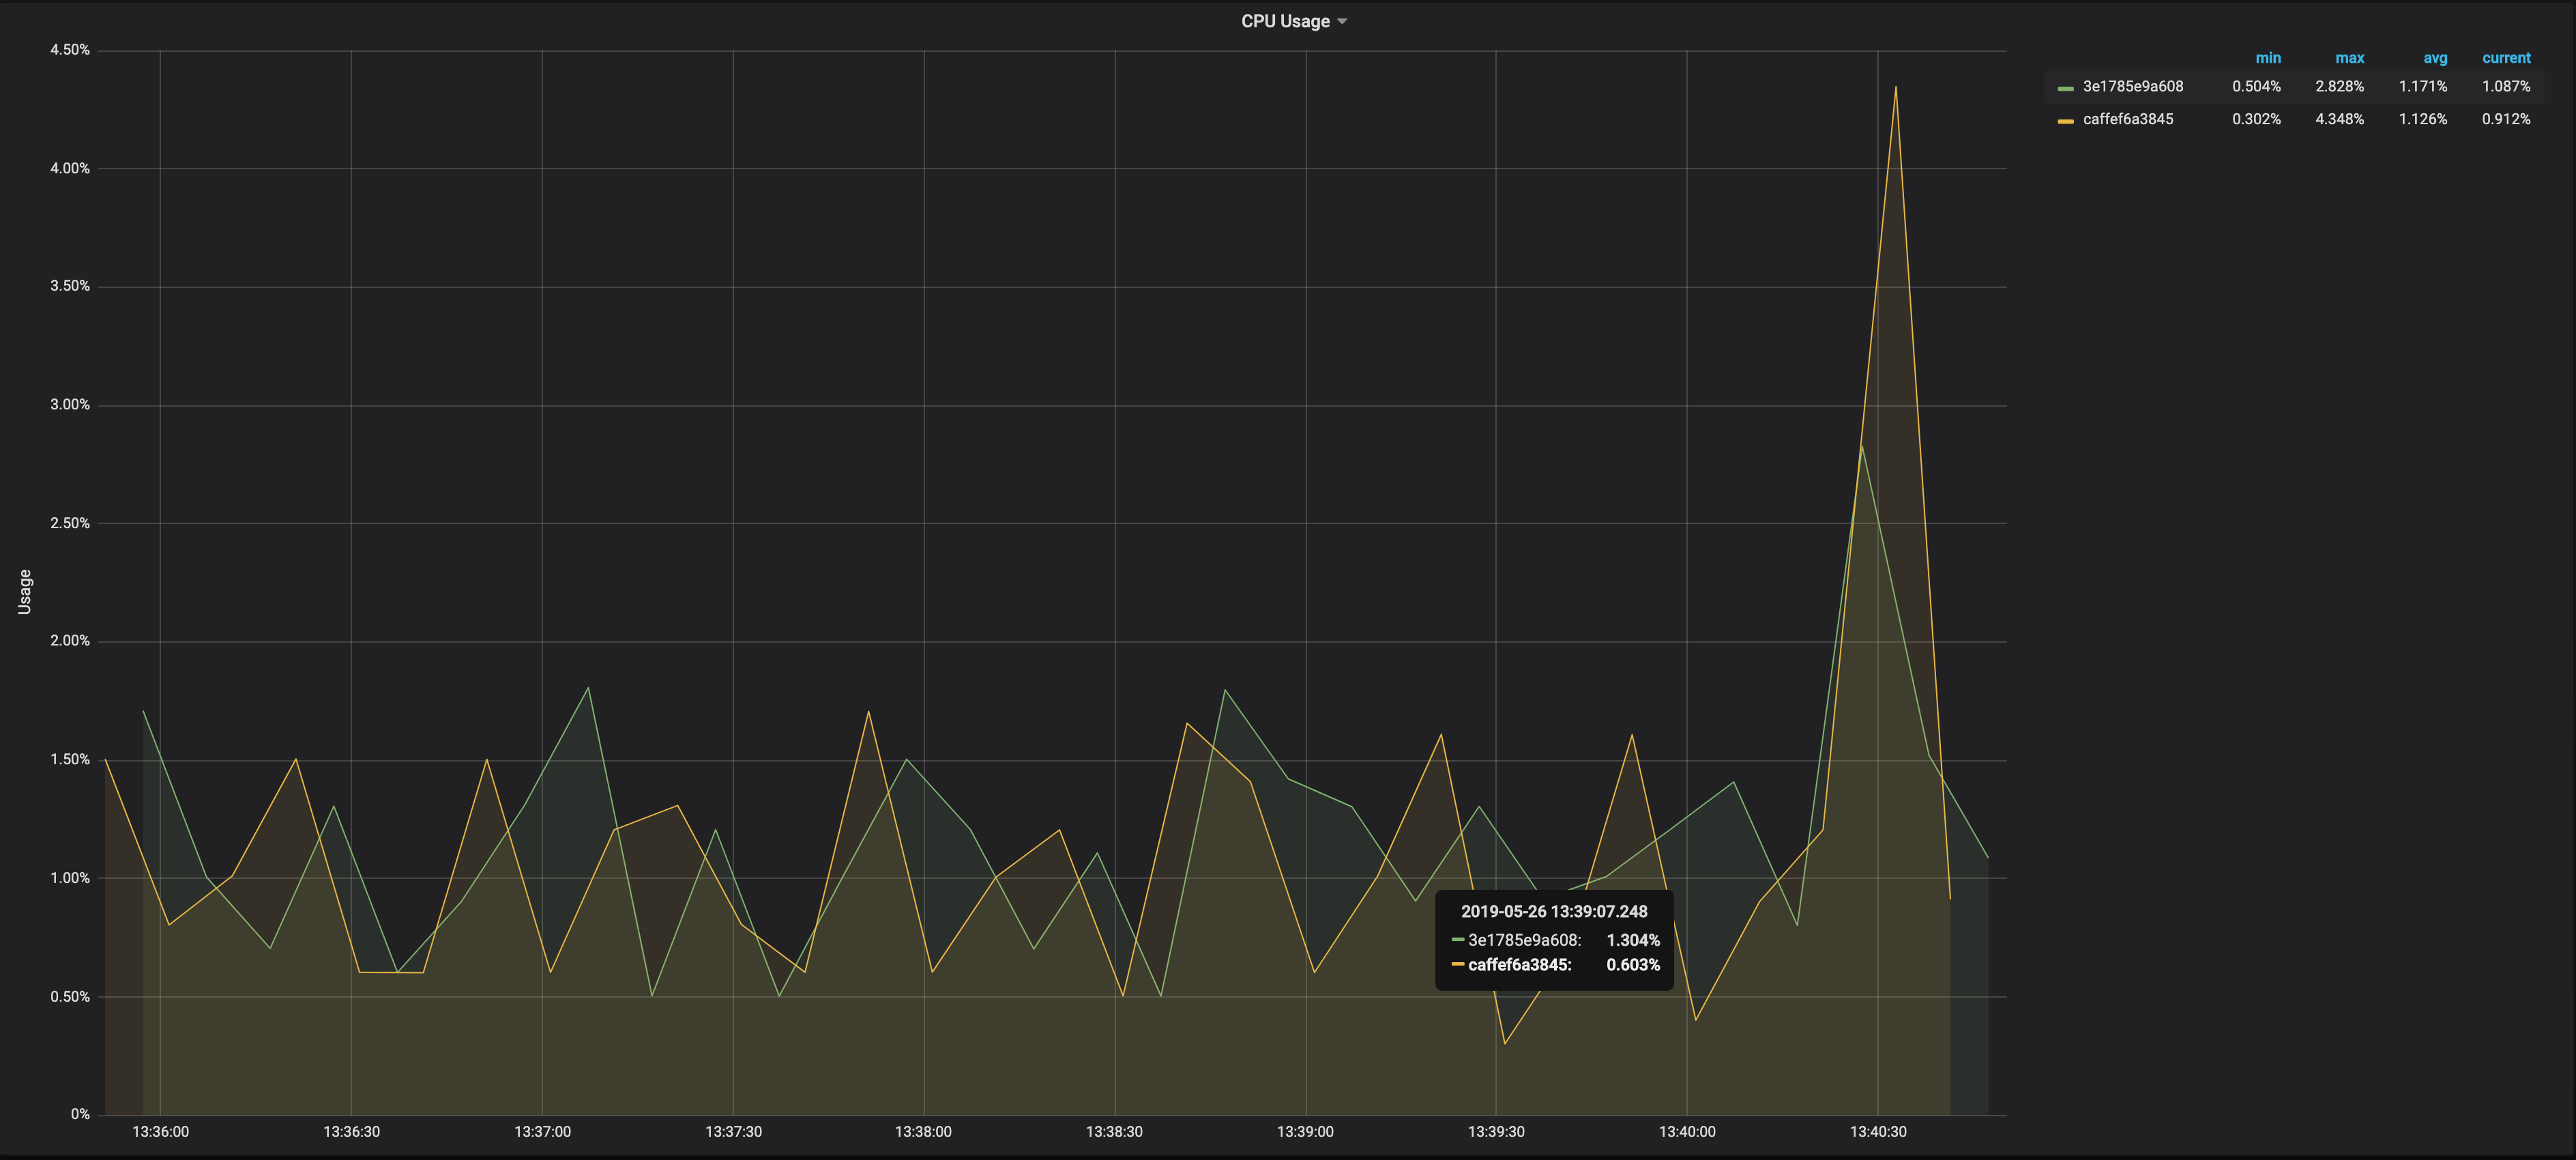
\includegraphics[width=\linewidth]{cpu.png}
	\caption{Processorverbruik-paneel}
	\label{fig:cpu}
\end{figure}

\section{Publicatie}
\label{sec:publication}

De package is ondertussen gepubliceerd op npm onder de naam \href{https://www.npmjs.com/package/express-influx-multilogger}{Express-influx-multilogger
}, alsook op \href{https://github.com/LeunensMichiel/express-influx-multilogger}{github}. Installatie en instructies kunnen gevonden worden in de README.md. 